\documentclass[beamer]{standalone}
\definecolor{printred}{RGB}{215,25,28}
\usepackage{tikz}
\usetikzlibrary{patterns}
\begin{document}
\newcommand{\drawstencil}[2]{%
  \draw[darkgray, thick, pattern=north west lines, pattern color=gray] (#1-1, #2) rectangle (#1+2, #2+1);
  \draw[darkgray, thick, pattern=north west lines, pattern color=gray] (#1, #2-1) rectangle (#1+1, #2+2);
  \draw[darkgray, thick, pattern=north east lines, pattern color=gray](#1, #2) rectangle (#1+1, #2+1);
}
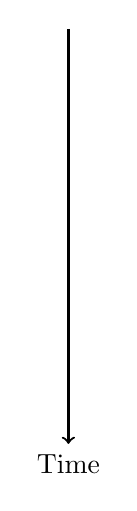
\begin{tikzpicture}[x=1.5em,y=1.5em]
  \draw[->, thick] (10,0) -- (10, -10) node (yaxis) [below] {Time};
%      \draw [<->,thick] (0,-10) node (yaxis) [above] {$y$}
%              |- (10,0) node (xaxis) [right] {$x$};
%
\end{tikzpicture}
\end{document}
